\documentclass[tcc,capa]{texufpel}
\usepackage{subcaption}
\usepackage[utf8]{inputenc} % acentuacao
\usepackage{graphicx} % para inserir figuras
\usepackage[T1]{fontenc}

\hypersetup{
    hidelinks, % Remove coloração e caixas
    unicode=true,   %Permite acentuação no bookmark
    linktoc=all %Habilita link no nome e página do sumário
}

\unidade{Centro de Engenharias}
\curso{Engenharia de Controle e Automação}
\nomecurso{Bacharelado em Engenharia de Controle e Automação}
\titulocurso{Bacharel em Engenharia de Controle e Automação}

\unidadeeng{Engineering Centre}
\cursoeng{Automation and Control Engineering}


\title{Análise de segurança em protocolos de comunicação IoT}

\author{Veiga}{Eduardo Santos da}
\advisor[Prof.]{Sigales}{Marlon Soares}

%Palavras-chave em PT_BR
\keyword{Cybersegurança}
\keyword{Internet-das-coisas}
\keyword{Protocolos-comunicação}
\keyword{SCADA}

%Palavras-chave em EN_US
\keywordeng{Cybersecurity}
\keywordeng{Internet-of-things}
\keywordeng{Communication-protocols}
\keywordeng{SCADA}

\begin{document}

%\renewcommand{\advisorname}{Orientadora}           %descomente caso tenhas orientadora
%\renewcommand{\coadvisorname}{Coorientadora}      %descomente caso tenhas coorientadora

\maketitle 

\sloppy

\fichacatalografica

%\folhadeaprovacao

%Composição da Banca Examinadora
\begin{aprovacao}{30 de fevereiro de 2019} %data da banca por extenso
\noindent Prof. Dr. Marilton Sanchotene de Aguiar (orientador)\\
Doutor em Computação pela Universidade Federal do Rio Grande do Sul.\\[1cm]

\noindent Prof. Dr. Paulo Roberto Ferreira Jr.\\
Doutor em Computação pela Universidade Federal do Rio Grande do Sul.\\[1cm]

\noindent Prof. Dr. Ricardo Matsumura Araujo\\
Doutor em Computação pela Universidade Federal do Rio Grande do Sul.\\[1cm]

\noindent Prof. Dr. Luciano da Silva Pinto\\
Doutor em Biotecnologia pela Universidade Federal de Pelotas.
\end{aprovacao}

%Opcional
\begin{dedicatoria}
  Dedico\ldots 
\end{dedicatoria}

%Opcional
\begin{agradecimentos}
  Agradeço ao mozy por ser um mozy
\end{agradecimentos}

%Opcional
\begin{epigrafe}
  Só sei que nada sei.\\
  {\sc --- Sócrates}
\end{epigrafe}

%Resumo em Portugues (no maximo 500 palavras)
\begin{abstract}
O termo Internet das Coisas (IoT) foi concebido em 1999 por Kevin Ashton para ilustrar o poder de conectar etiquetas de RFID (Radio Frequency Identification - \textit{Identificação por Radiofrequência}) na internet para gerenciamento de cadeia de suprimentos \cite{ashton}. Desde então, várias definições evoluíram baseadas nas definições das tecnologias em voga no momento, porém, todas falando de uma rede feita de máquinas, para máquinas - a rede \textit{machine-to-machine} (M2M). Devido a heterogeneidade de dispositivos numa rede IoT, se faz necessário uma estrutura bem desenvolvida, capaz de prover a segurança exigida para os dados recolhidos de sensores. 

Uma solução ampla de segurança é de difícil implementação na camada de rede e percepção definida na arquitetura descrita por \cite{xu}, uma vez que os dispositivos instalados nessa camada são de baixo poder computacional, incapazes de prover soluções de criptografia. É justamente nessa camada onde o maior risco à infraestrutura de uma solução IoT se apresenta, uma vez que essa baixa potência computacional é acompanhada de protocolos de comunicação simples e vulneráveis.
\end{abstract}

%Resumo em Inglês (no maximo 500 palavras)
\begin{englishabstract}{Security Analysis in IoT Communication Protocols}

The Internet of Things as a term was first coined in 1999 by Kevin Ashton to better illustrate the potential in connecting several RFID tags on the internet for supply chain management \cite{ashton}. Since then, several definitions of the Internet of Things evolved based on the latest technology en vogue. However, all of those definitions speak of a network made by machines, for machines - the machine-to-machine network (M2M). Due to the calleidoscope of different devices one can use to create an IoT network, there is a need for a well understood framework capable of providing the security demanded by the usually sensitive nature of the data harvested by the sensors.

An all-encompassing safety solution is hard to implement in the network and perception layers as defined by the framework described by \cite{xu}, since the devices on this layer are usually weak on computing power, which hinders their ability to include cryptography and secure pipes for communications. Its exactly on this junction where the biggest risk to the infrastructure lies, since the simplicity of the end-devices usually means simplistic and vulnerable communications protocols.
\end{englishabstract}

%Lista de Figuras
\listoffigures

%Lista de Tabelas
\listoftables

%lista de abreviaturas e siglas
\begin{listofabbrv}{LoRaWAN}%coloque aqui a maior sigla para ajustar a distância
        \item[ABNT] Associação Brasileira de Normas Técnicas
        \item[SCADA] Supervisory Control and Data Acquisition - \textit{Controle Supervisório e Aquisição de dados}
        \item[IoT] Internet of Things - \textit{Internet das Coisas}
        \item[ICMP] Internet Control Message Protocol - \textit{Protocolo para Mensagens de Controle via Internet}
        \item[TCP] Transmission Control Protocol - \textit{Protocolo de controle de transmissão}
        \item[UDP] User Datagram Protocol - \textit{Protocolo de datagramas de usuário}
        \item[VPN] Virtual Private Network - \textit{Rede Privada Virtual}
        \item[UTM] Universal Threat Manager - \textit{Gerenciador Universal de Ameaças}
        \item[SSH] Secure Shell - \textit{Túnel de Comunicação Segura}
        \item[ARP] Address Resolution Protocol - \textit{Protocolo de Resolução de Endereços}
        \item[DNS] Domain Name Server - \textit{Servidor de Nome de Dominio}
        \item[IIoT] Industrial Internet of Things - \textit{Internet das coisas Industriais}
        \item[IoMT] Internet of Medical Things - \textit{Internet das coisas médicas}
        \item[IoE] Internet of Everything - \textit{Internet de Tudo}
        \item[M2M] Machine-to-Machine - \textit{Comunicação máquina a máquina}
        \item[LPWAN] Low-Power Wide-Area Network - \textit{Rede de Grande Área e Baixa Potência}
        \item[LoRaWAN] Long-Range Wide Area Network - \textit{Rede Grande Área e Longo Alcance}
        \item[NBIoT] Narrowband Internet of Things - \textit{Internet das coisas em banda estreita}
        \item[BLE] Bluetooth Low Energy - \textit{Protocolo Bluetooth de Baixa Energia}
        \item[RFID] Radio Frequency Identification - \textit{Identificação por Radiofrequência}
        \item[NFC] Near Field Communication - \textit{Comunicação em campo próximo}
        \item[WLAN] Wireless Local Area Network - \textit{Rede Local sem-fio}
        \item[MQTT] Message Queuing Telemetry Transport - \textit{Transporte Enfileirado de Mensagens de Telemetria}
        \item[CoAP] Constrained Application Protocol - \textit{Protocolo de Aplicação Limitada}
        \item[LAN] Local Area Network - \textit{Rede local}
        \item[WAN] Wide Area Network - \textit{Rede ampla}
        \item[DHCP] Dynamic Host Configuration Protocol - \textit{Protocolo de configuração de hóspede dinâmico}     
\end{listofabbrv}

%Sumario
\tableofcontents

\chapter{Introdução}

Com a alvorada da era da informação, nossa existência tem sido cada vez mais coberta por um vapor de dados. A popularização dos smartphones desde o lançamento do iPhone em 2006 e a ampla adoção do equipamento em meados de 2013, somado aos avanços em miniaturização de sensores e potência computacional dos últimos 20 anos nos fizeram mergulhar num mar de informação sem precedentes. Com a ubiquidade desses dispositivos e sensores, o estado de interconexão se espalha tal qual uma teia de uma aranha em uma casa abandonada. 

Essa tecnologia é amplamente explorada na indústria muito antes de estar disponível para o usuário final, sob o conceito de SCADA (traduzindo livremente, controle supervisório e aquisição de dados), que é pesquisado e melhorado desde a década de 1970, quando os primeiros sistemas de controle computadorizados eram usados para monitorar processos industriais. A coalescência concomitante da computação industrial e doméstica permite amplos modelos de sistemas, independente do contexto.

E é exatamente nesse cenário de informação ubíqua e interconectividade extensiva que se oriunda a Internet das Coisas (\textit{IoT - Internet of Things}), junto com a necessidade de proteger esses dispositivos e seus dados, seja com a miríade de informações disponíveis em um \textit{smartphone} ou em um sistema de automação doméstica. E de maneira mais crítica, a produção ou segurança nacional implicada em uma planta industrial é de extrema prioridade de proteção. 

\section{Stuxnet}

Para ilustrar a importância da proteção de plantas industriais e sistemas SCADA, pode-se analisar a história de um dos vírus do tipo \textit{worm} mais potentes da história recente - o Stuxnet.

O stuxnet era um \textit{worm} segmentado \cite{stuxnet_kaspersky}, que era espalhado em dispositivos USB (pen-drives) e computadores Windows. O vírus buscava em cada computador infectado por sinal de software do Siemens Step 7, utilizado por computadores industriais agindo como CLPs (Computador Lógico-Programável) controlando e monitorando equipamentos eletromecânicos. Depois de encontrar um CLP, o \textbf{worm} atualizava seu código pela internet e começava a enviar instruções mal-formadas para o equipamento eletromecânico (centrífugas nucleares para enriquecimento de urânio) e ao mesmo tempo, respostas falsas ao controlador principal. Qualquer pessoa monitorando o equipamento não teria ideia de que algo de errado estaria acontecendo até que o equipamento começasse a se auto-destruir.

\begin{quote}
 Antes do Stuxnet, ninguém pensava na cibersegurança dos sistemas industriais. Se presumia que o isolamento das redes industriais era uma medida suficiente para preservar a segurança empresarial. Através do ataque à máquinas desconectadas, os criadores do \textit{worm} inauguraram uma nova era na segurança da informação. A importância do Stuxnet pode ser comparado apenas com o Morris Worm , criado em 1988.

 - \citeauthor{stuxnet_kaspersky}, 2014
\end{quote}

\section{A ponta da lança}

Os estudos desenvolvidos por \citet{smart_cities} sugerem várias aplicações da internet das coisas, como redes inteligentes, aprimoramentos na gestão de energia, telemedicina, veículos inteligentes, etc. Esses campos se dispõe num paradigma urbano de IoT para melhorar os serviços públicos de manutenção, vigilância e segurança. De acordo com os autores, o emprego de IoT urbano tem o potencial de otimizar o gerenciamento de serviço público, principalmente através da análise da quantidade de dados para promover governança transparente e eficiente. 

A evolução sistemática do conceito de IoT e o acompanhamento em vários domínios desenvolvido por \citet{Ibarra-Esquer} nos mostra como idealmente, é essencial ter uma infraestrutura composta de dispositivos de sensoriamento, enlaces de comunicação e aplicações destinadas ao usuário final para ter um ambiente inteligente. No entanto, não é de forma alguma essencial dispor de toda a infraestrutura no começo \cite{laya}. Uma solução única não pode acomodar as aplicações de um campo heterogêneo como a IoT, não obstante a falta de serviços de segurança e ampla gama de dispositivos, bem como as preocupações com privacidade do usuário final. 

Com a iminente ubiquidade de uma rede de máquinas construída com os conceitos de IoT, faz-se necessário um olhar com cuidado sobre a segurança empregada, devido a natureza sensível das informações que trafegam nessa rede. Assim, será feito uma extensiva revisão bibliográfica de todos os conceitos importantes para essa análise, seguido de um mapeamento dos protocolos mais utilizados e uma análise de segurança através de várias técnicas de invasão. Por fim, os resultados dessas informações serão discutidos na tentativa de encontrar um paradigma seguro para uma rede IoT.

\chapter{Revisão Bibliográfica}

\section{Redes de Computador}
\subsection{Modelo OSI}

Segundo \citet{kurose}, o modelo OSI é um modelo conceitual, desenvolvido pela Organização de Padronização Internacional (ISO) que permite sistemas diversos se comunicarem usando protocolos. Foi o primeiro modelo padrão para comunicação em rede, adotado por todas as grandes companhias de computação e telecomunicação desde a década de 1980.

Apesar da internet moderna não ser estritamente baseada no modelo OSI, e sim no modelo TCP/IP mais simples, \citet{kurose} mostra que o modelo OSI ainda é amplamente usado, uma vez que permite visualizar como redes de computador operam, e serve como um guia para auxiliar isolar e 
diagnosticar condições anormais.

De acordo com \citet{imperva}, as vantagens do modelo OSI são, entre outras:
\begin{itemize}
    \item Determinar o hardware e software necessários para construir a rede;
    \item Entender e comunicar o processo seguido por componentes comunicando através de uma rede;
    \item Realizar diagnósticos, identificando qual camada de rede está causando problemas;
    \item Definir qual partes da rede um produto vai agir.
\end{itemize}

\begin{figure}[h]
    \centering
    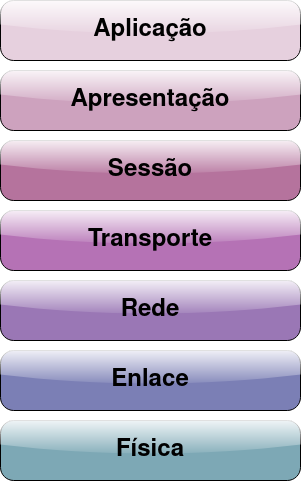
\includegraphics[scale=0.4]{figs/osi.png}
    \medskip
    \caption{Visualização do modelo OSI, modificado de \cite{kurose}}
    \label{fig:osi}
\end{figure}

\subsubsection{Camada 1: Física}

Essa camada inclui o equipamento físico envolvido na transferência de dados, como cabos, \textit{switches} de rede e fibras óticas \cite{cloudflare_layers}. É aqui que os dados são convertidos em uma transmissão de dígitos binários.

\subsubsection{Camada 2: Enlace}

A camada de enlace estabelece e termina a conexão entre dois nós fisicamente conectados numa rede. A camada de rede é dividida em duas partes \cite{imperva}: 
    \begin{itemize}
        \item Controle Lógico de Enlace (LLC), responsável pela sincronia de quadros, realiza correção de erros e identifica protocolos de rede;
        \item Controle de Acesso de Meio (MAC), responsável por conectar e endereçar dispositivos e definir permissões para transmitir e receber dados
    \end{itemize}

\subsubsection{Camada 3: Rede}

De acordo com \citet{cloudflare_layers}, a camada de rede é responsável por facilitar a comunicação entre duas redes diferentes. Se dois dispositivos em comunicação estiverem na mesma rede, a camada então é redundante. A facilitação de comunicação ocorre \citet{cloudflare_layers} pela fragmentação de segmentos da camada de transporte em unidades menores, chamadas de pacotes, no dispositivo remetente, e remontando esses pacotes no dispositivo receptor. A camada de rede também é responsável pelo roteamento de dados da origem, utilizando endereços de rede (tipicamente, endereços IP), até o destino.

\subsubsection{Camada 4: Transporte}

A camada de transporte é responsável pela comunicação ponta a ponta entre os dois dispositivos. A explicação apresentada em \citet{kurose} nos mostra que os protocolos de camada de transporte provém \textit{comunicação lógica} entre processos de aplicações rodando em computadores diferentes numa mesma rede. Ou seja, como se os diferentes computadores rodando os processos estivessem diretamente conectados, independente da distância física ou tipo de conexão intermediária, que é tratada pelas camadas inferiores

\subsubsection{Camada 5: Sessão}

A camada de sessão cria canais de comunicação (sessões) entre dispositivos. Conforme mostrado por \citet{imperva}, é necessário que as sessões se mantenham abertas enquanto dados estão sendo transferidos. A camada de sessão também é responsável por sincronizar os dados por pedaços. O exemplo mostrado por \citet{cloudflare_layers} nos ajuda a ilustrar a utilidade: se um arquivo de 100 megabytes está sendo transferido, a camada de sessão pode criar pedaços de 5 megabytes. Assim, se a conexão for interrompida durante a transferência, ela pode ser reiniciada no último pedaço.

\subsubsection{Camada 6: Apresentação}

Como descrito em \citet{cloudflare_layers}, dois dispositivos em comunicação devem estar usando métodos de codificação diferentes, portanto camada de apresentação, de acordo com \citet{imperva}, prepara os dados para a camada de aplicação e define como dois dispositivos devem encodificar, criptografar e comprimir dados de maneira a ser recebido corretamente na outra ponta. 

\subsubsection{Camada 7: Aplicação}

De acordo com \citet{cloudflare_layers}, a camada de aplicação é a única camada que interage diretamente com os dados do usuário. Aplicações como os navegadores dependem da camada de aplicação pra iniciar a comunicação. No entanto, é necessário lembrar que essas aplicações não fazem parte da camada de aplicação, mas sim, \citet{cloudflare_layers} mostra que a camada de aplicação é responsável pelo protocolo e manipulação de dados que o software depende para apresentar dados significativos para o usuário. Protocolos da camada de aplicação incluem, por exemplo, de acordo com \citet{imperva}, o HTTP, FTP, POP, SMTP e DNS.


\subsection{Modelo OSI vs Modelo Internet (TCP/IP)}

O modelo TCP/IP ajuda a determinar como um computador deve se conectar a internet e como dados podem ser transmitidos. Esse modelo ajuda a criar uma rede virtual quando múltiplos computadores estão conectados mutualmente \cite{cloudflare_layers}. A diferença chave é que o modelo TCP/IP é mais simples, simplificando várias camadas em uma, a saber:
\begin{itemize}
    \item Camadas 7, 6 e 5 da OSI são combinadas na camada de Aplicação TCP/IP;
    \item Camadas 1 e 2 são combinadas na camada de acesso de rede TCP/IP;
\end{itemize}

Outra diferença importante é a especificação dos modelos \cite{imperva}. O modelo TCP/IP é funcional e feito pra resolver problemas específicos de comunicação, e é baseado em protocolos padronizados e específicos. Em contrapartida, o modelo OSI é genérico e independente de protocolos, feito para descrever todas as formas de comunicação em rede. No mesmo tom, no modelo TCP/IP, a maioria das aplicações usam todas as camadas, enquanto no modelo OSI, aplicações simples não usam todas as 7 camadas. No modelo OSI, apenas as camadas 1, 2 e 3 são mandatórias para permitir comunicação de dados

\subsection{Topologias}
Redes de comunicação existem em diferentes sabores, que podem ser divididos em redes físicas e lógicas. Atualmente, robustez e escalabilidade são de caráter essencial, portanto, a ênfase é posta no design de topologia lógico \cite{schiller}. As topologias de rede podem ser resumidas em quatro grandes grupos, incluindo o papel específico de nós do tipo \textit{gateway} (portal), uma vez que esses nós mostram impactos diferentes em vários cenários em IoT.
\begin{figure}[h]
\begin{subfigure}{.24\textwidth}
  \centering
  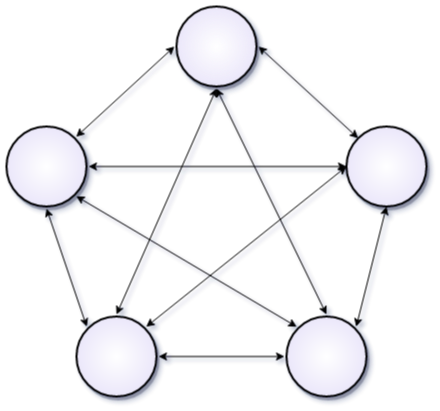
\includegraphics[width=.8\linewidth]{figs/mesh.png}
  \caption{Topologia Malha (mesh)}
  \label{fig:mesh}
\end{subfigure}%
\begin{subfigure}{.24\textwidth}
  \centering
  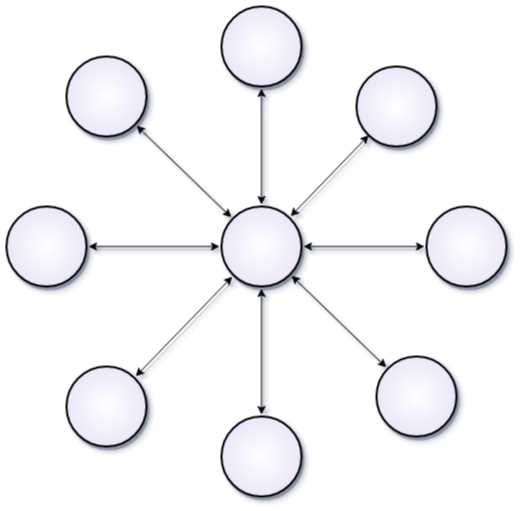
\includegraphics[width=.8\linewidth]{figs/star.png}
  \caption{Topologia Estrela}
  \label{fig:star}
\end{subfigure}
\begin{subfigure}{.24\textwidth}
  \centering
  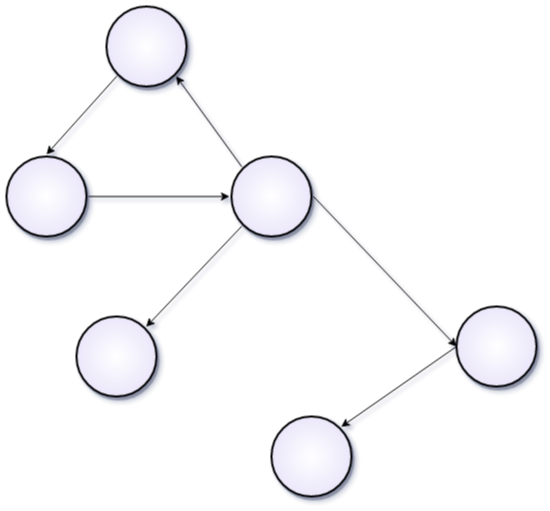
\includegraphics[width=.8\linewidth]{figs/pmesh.png}
  \caption{Topologia Malha Parcial}
  \label{fig:pmesh}
\end{subfigure}
\begin{subfigure}{.24\textwidth}
  \centering
  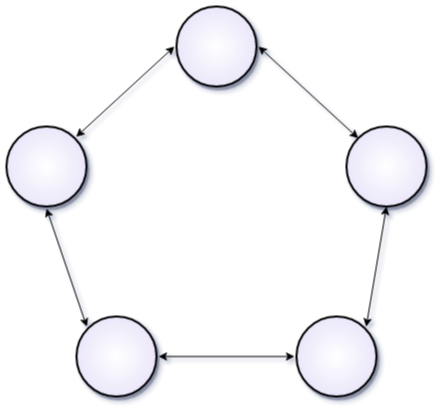
\includegraphics[width=.8\linewidth]{figs/dchain.png}
  \caption{Topologia Ciranda}
  \label{fig:dchain}
\end{subfigure}
\caption{Topologias de rede, adaptado de \cite{schiller}}
\label{fig:topo}
\end{figure}

\subsubsection{Conexão ponto-a-ponto}

Nós ligados com uma conexão dedicada formam uma topologia ponto a ponto \cite{schiller}, onde nós agem como pontos finais. De maneira a funcionar  corretamente, nem um dos pontos nem o enlace pode falhar.

\subsubsection{Ciranda}

Quando nós são ligados em série, a rede resultante é conhecida como ciranda (ou, cadeia de margaridas). Uma rede linear conecta cada nó ponto-a-ponto, onde um nó pode funcionar como um monitor IoT \cite{schiller}.  Geralmente é utilizada em redes menores devido a baixo custo de instalação. No entanto, é uma topologia complexa de diagnosticar, uma vez que uma perturbação em um nó pode se propagar para toda a rede.

\subsubsection{Estrela}

Quando todos os nós estão conectados a um \textit{gateway} central, a topologia resultante é chamada de topologia estrela. As vantagens principais são a efetividade de custo, facilidade de instalação e resiliência \cite{schiller}. Falha ou vulnerabilidade de um nó não compromete toda a rede.

\subsubsection{Malha}

Uma topologia de malha (\textit{mesh}) é caracterizada por pelo menos três nós distintos, onde cada um desses pontos é vizinho de um conjunto de outros nós, conforme ilustrado na figura \ref{fig:mesh}. Essas conexões podem ser geradas de maneira dinâmica ou hierárquica.

\subsubsection{Nós \textit{Gateway}}

\section{Preocupações com Segurança} 

O termo \textit{Segurança da Informação} não tem uma definição estática e evolui conforme a tecnologia existente também o faz. Porém, desde a década de 80, a segurança da informação engloba as metas de garantir a disponibilidade, confidencialidade e integridade da informação \cite{schiller}. Assim, vamos definir os seguintes axiomas:

\begin{itemize}
    \item Uma mensagem é confidencial se, e somente se, apenas o remetente e o destinatário sabem da sua existência
    \item Uma mensagem é integra apenas se o conteúdo é idêntico entre o remetente e o destinatário.
    \item Uma mensagem tem disponibilidade se é legível pelo remetente e o destinatário a qualquer momento
    \item Uma mensagem deve ser capaz de demonstrar a sua origem e vice versa
    \item Uma mensagem não pode ser enviada com o remetente adulterado
\end{itemize}

\subsection{Terminologia de segurança}

A terminologia de segurança descrita por \citet{schiller} cria um terreno comum para análise de segurança, definindo o conceito de \textit{adversário}, \textit{malware}, \textit{risco}, \textit{ameaça} e \textit{vulnerabilidade}:

\begin{itemize}
    \item Um \textit{Adversário} é definido como uma entidade acessando os recursos do sistemas de maneira ilegítima;
    \item Um \textit{Malware} é a ferramenta em software que atinge o objetivo do adversário
    \item Uma \textit{Ameaça} é qualquer evento tendo o potencial de violar a segurança e causar dano. Sua existência requer capacidade de execução ou circunstâncias favoráveis. Por exemplo, um \textit{malware} instalado por um \textit{adversário} sempre configura uma ameaça, mas nem sempre se torna um \textit{Risco}
    \item Uma \textit{Vulnerabilidade} existe quando uma falha no ponto de design, implementação, operação ou gerenciamento acontece.
    \item \textit{Risco} ocorre quando uma ameaça e uma vulnerabilidade se encontram.
\end{itemize}

Quando todas as pré-condições supracitadas são executadas, esse \textit{Risco} vira um \textit{Ataque}. Um ataque pode ter como objetivo alterar recursos do sistema ou adquirir informação.

\section{Internet das Coisas}

O avanço tecnológico, no passado recente, transformou a internet para uma rede onde tudo é ligado e objetos de uso cotidiano podem ser reconhecidos e controlados. A internet das coisas é uma rede de objetos físicos que podem fazer sensoriamento, comunicação e serem acessados através da internet, tornando-se parte integral da mesma \cite{Sharma2019}. Esses objetos são embarcados com eletrônicos, \textit{software}, sensores, atuadores e a conectividade de rede que habilita-os a coletar e trocar seus dados usando vários protocolos. Portanto, \cite{Sharma2019} nos diz que a IoT oferece conectividade de serviços, dispositivos e sistemas que vão além da comunicação Máquina-Máquina (M2M) e está disposto a receber aplicações em domínios diferentes.

\subsection{Uma breve contextualização histórica}

O termo Internet das Coisas foi concebido em 1999 por Kevin Ashton para ilustrar o poder de conectar etiquetas de RFID na internet para gerenciamento de cadeia de suprimentos \cite{ashton}. Desde então, várias definições evoluíram baseadas nas definições das tecnologias em voga no momento e na gama de aplicações possíveis. Diferentes pesquisadores e cientistas definem o termo de maneiras diferentes, porém, a definição utilizada aqui é que a IoT é uma constelação de objetos, tecnologias, dispositivos e protocolos conectados por uma estrutura unificada que inclui computação ubíqua, computação em nuvem, análise de dados e visualização.

Com a taxa de crescimento exponencial da IoT, o campo industrial está amplamente motivado para investir com o objetivo de melhorar processos, minimizar riscos e melhorar experiência do usuário \cite{Sharma2019}. No entanto, IoT não é só colocar um sensor num objeto e chamá-lo de "inteligente". Uma solução compreensiva de IoT precisa de uma infraestrutura apropriada e um ambiente de apoio para a coleção e análise de dados. Se não existir um estudo intenso do ponto de vista de sistemas, se torna extremamente complexo entender as tecnologias chave de IoT \cite{xu}. Sendo assim, é necessário primeiro estruturar essas tecnologias.

\subsection{O modelo de seis camadas da IoT}

A arquitetura existente da internet foi adotada quatro décadas atrás, na forma de protocolos TCP/IP, mas hoje é incompatível para servir a rede imensa que a IoT necessita. Portanto, é necessário existir uma arquitetura nova que consiga trabalhar com uma rede de mais de 25 bilhões de dispositivos conectados \cite{Sharma2019}. Essa nova arquitetura deve usar protocolo de código aberto para suportar aplicações de redes já existente e prover segurança e qualidade de serviço. Portanto, várias arquiteturas de segurança para IoT são propostas. \citet{xu} propôs uma arquitetura em seis camadas baseada numa estrutura hierárquica e desenvolvidas no contexto de uma rede RFiD, ilustradas na Figura \ref{fig:6layer}. Para este trabalho, serão consideradas para análise apenas as camadas de rede, percepção e aplicação. 

\subsubsection{Primeira camada: Codificação}
    Essa é a camada base da arquitetura IoT, onde cada objeto de interesse é fornecido com um código para identificação única.

\subsubsection{Segunda camada: Percepção}
    O objeto de interesse com código único é atribuído com significado físico, através da conexão de dispositivos IoT. Os dispositivos geralmente são sensores como etiquetas RFID, sensores infravermelhos ou outros sensores. Nessa camada, os sensores recolhem a informação do objeto de interesse, convertendo para sinal digital e passados adiante para a camada de rede \footnote{não confundir com a camada OSI homônima}.

\subsubsection{Terceira camada: Rede}
    A camada de rede é responsável pela transmissão segura de dados entre a camada de percepção e a camada de \textit{middleware}, onde ocorre o processamento. Essa camada pode utilizar vários meios de transmissão como Bluetooth, WiMaX, Zigbee, GSM, 3G, com protocolos como IPv4, IPv6, MQTT, AMQP, CoAP, XMPP, DDS e etc, e serve como um ponto de inflexão entre a internet e a rede baseada em comunicação.

\subsubsection{Quarta camada: \textit{Middleware}}
    Essa camada usa tecnologias avançadas como computação ubíqua, computação em nuvem para acessar uma base de dados diretamente e armazenar e prover as informações necessárias. Essa camada principalmente processa os dados de sensores recebidos pela camada de rede e executa uma ação automatizada baseada no resultado.

\subsubsection{Quinta camada: Aplicação}
    Essa camada entrega serviços personalizados baseado nas necessidades do usuário, usando o resultado dos dados processados.

\subsubsection{Sexta camada: Negócios}
    A camada de negócios é a camada superior da arquitetura IoT, onde várias regras de negócio são geradas para estratégias efetivas. As aplicações e serviços disponibilizados pela IoT são gerenciados nessa camada.

\begin{figure}[h]
    \centering
    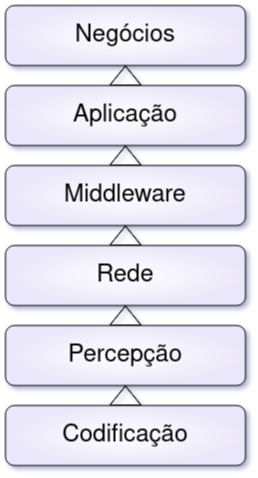
\includegraphics[scale=0.5]{figs/xu.png}
    \caption{Arquitetura de 6 camadas proposta por \citet{xu}}
    \label{fig:6layer}
\end{figure}



\subsection{Protocolos}

\subsubsection{TCP/IP}
O Protocolo de Controle de Transmissão E Protocolo de Internet (TCP/IP) é o protocolo mais amplamente utilizado na internet e quebra uma mensagem em pacotes para transmissão.

Vários problemas na arquitetura TCP/IP devem ser considerados no contexto de IoT \cite{schiller}. Entre eles, a unidade máxima de transmissão (MTU) de 1280 bytes, que pode ser grande demais para dispositivos de baixa potência. De maneira semelhante, o TCP oferece várias utilidades como confiança de transmissão, controle de fluxo e capacidade de evitar congestionamentos, que podem ser pesadas demais para implementação em dispositivos IoT. Ademais, vias de comunicação implementadas em IoT podem ter perdas na comunicação que não são compensadas com os controles de fluxo previstos no TCP, uma vez que o TCP sempre trata perdas como sendo causadas por congestionamento na rede. Esses listados são apenas alguns disponíveis no mercado, sendo o MQTT e o CoAP mais comuns.

\subsubsection{6LoWPAN}

A Força Tarefa de Engenharia de Internet (IETF - \textit{Internet Engineering Task Force}) criou um grupo de trabalho denominado \textit{IPv6 over Low-Power Wireless Personal Area Networks} (IPv6 sobre redes sem fio pessoais de baixa potência), abreviado como 6LoWPAN. Esse protocolo implementa funcionalidade IPv6 sobre protocolo UDP para garantir que nós sensores sejam compatíveis com diversas camadas físicas e MAC \cite{schiller}

\subsubsection{Thread}
Dispositivos prontos para protocolo Thread suportam um conjunto do padrão IEEE 802.15.4 e fazem uma implementação da 6LoWPAN \cite{schiller}. Devido ao baixo consumo de energia, dispositivos IoT tem um sinal fraco de transmissão, fazendo a comunicação ser mais difícil Portanto, o Datagram Transport Layer Security (DTLS - \textit{Segurança da Camada de Transporte por Datagramas}) é utilizado no Thread para garantir confidencialidade da mensagem.

\subsubsection{MQTT / CoAP}

o Protocolo Limitado de Aplicação (\textit{CoAP - Constrained Application Protocol})  e o Transporte de Mensagens de Telemetria Enfileirada (\textit{MQTT - Message Queuing Telemetry Transport}) são os dois principais protocolos de mensagem na camada de transporte usado em IoT \cite{schiller}. Ambos protocolos foram desenvolvidos para trabalhar com dispositivos IoT de baixa potência. O CoAP é um protocolo na camada de serviço feito para dispositivos de internet com recursos limitados, como redes de sensores sem fio, com a intenção de simplificar a funcionalidade do HTTP \textit{(Hypertext Transfer Protocol - Protocolo de Transferência de Hipertexto}) e adaptar pra aplicações de IoT ao aumentar a simplicidade. Já o MQTT é um protocolo de mensagem do tipo assinatura/publicação para conectar dispositivos embarcados através de um servidor (chamado \textit{broker}), onde as mensagens são endereçadas para tópicos aos quais os demais clientes assinados conseguem receber.

\subsubsection{Grafana}

O Grafana é uma das arquiteturas mais populares para receber dados de dispositivos IoT \cite{schiller}, ela utiliza o protocolo MQTT atrelado à plataforma de código aberto Graphite e um sistema de visualização, que pode pegar dados em série temporal e exibi-los de forma amigável.

\subsubsection{AMQP}

o Protocolo Avançado de Fila de Mensagens \textit{(AMQP - Advanced Message Queue Protocol)} foi feito para prover mensagens de alta performance e uso geral, com disponibilidade de implementação de filas e roteamento complexo \cite{o2007toward}, resultando num protocolo capaz de fazer rotinas de entrega mais complexa como multicast.

\chapter{Metodologia}

Devido a natureza polimórfica de sistemas de Internet das Coisas, uma análise de segurança requer como primeiro passo uma análise profunda de \textit{hardware}, \textit{software} e de rede. Para cobrir essas camadas, é necessário conduzir uma análise de vulnerabilidade em potencial no sistema como, por exemplo, \textit{software} desatualizado, comunicação insegura, ou senhas fracas que podem ser exploradas.

De maneira semelhante, os sistemas de autenticação (LDAP, TACACS+, e semelhantes) devem ser analisados para garantir que mecanismos de autorização e controle de acesso como autenticação em múltiplos fatores estejam íntegros.

A parte mais vulnerável na maioria dos sistemas de IoT é a segurança da comunicação dos dispositivos de onde os dados são coletados, uma vez que nem sempre esses dispositivos possuem a capacidade computacional para implementar modos seguros de comunicação. Por exemplo, um sensor que transmite seus dados via wi-fi em texto aberto, ou com uma criptografia fraca. Por exemplo, a aplicação de uma criptografia TLS em uma plataforma ESP32 consome cerca de 17 vezes mais energia do que uma transmissão sem criptografia \cite{fischer}.

A abordagem mais extensiva de um \textit{pentest} envolve não só todos os passos supracitados como o desenvolvimento de uma descrição completa do sistema, a fim de compreender a área de superfície da penetração a ser executada e onde aplicar cada técnica. As técnicas e ferramentas variam, abaixo listam-se algumas: 

\begin{itemize}
    \item Ferramentas de mapeamento de rede e portas, como o nmap
    \item Analisadores de vulnerabilidade, como Nessus ou OpenVAS;
    \item Formalismos de exploração, para automatizar a exploração de vulnerabilidades descobertas
    como o Metasploit ou CANVAS
    \item Engenharia reversa em \textit{firmwares} e executáveis, procurando vulnerabilidades como um \textit{buffer overflow}, usando ferramentas como o IDA Pro, radare2 ou Binary Ninja
    \item Fuzzing, que é a técnica baseada em procurar vulnerabilidades através do envio de quantidades grandes de dados inesperados, aleatórios ou mal-formatados para o sistema, a fim de testar as rotinas de validação de entrada do sistema sob teste.
\end{itemize}

\begin{figure}[h]
    \centering
    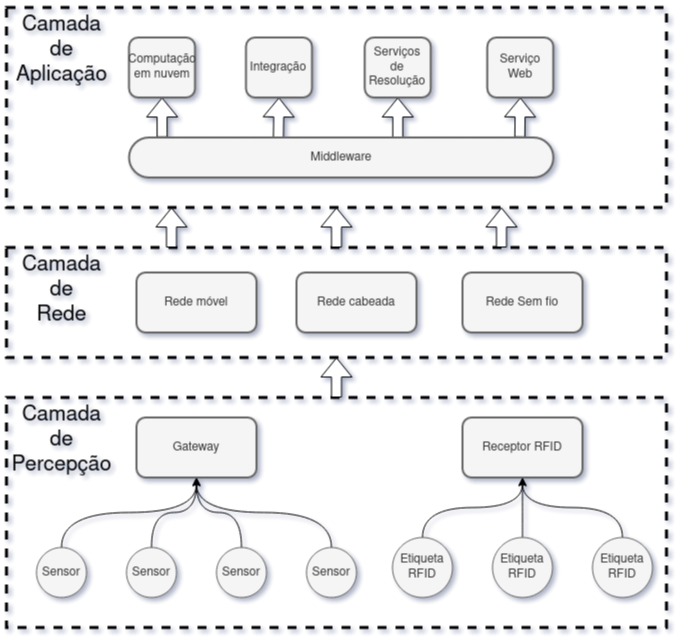
\includegraphics[scale=0.6]{camadas.png}
    \caption{Uma aplicação teórica, ilustrando as camadas sob análise. Adaptado de \cite{schiller}}
    \label{fig:layers}
\end{figure}


\chapter{Comparação de Protocolos de Mensagem}

De acordo com \citet{choice}, os quatro protocolos mais aceitos para troca de mensagem em infraestruturas IoT são o MQTT, CoAP, AMQP e HTTP. O quadro


% Please add the following required packages to your document preamble:
% \usepackage{graphicx}

\chapter{Análise de Resultados}
\chapter{Conclusão}

\bibliographystyle{abnt}
\bibliography{bibliografia} 

% Apêndices (Opcional) - Material produzido pelo autor
\apendices
\chapter{Um Apêndice}

% Anexos (Opcional) - Material produzido por outro
\anexos
\chapter{Um Anexo}


\chapter{Outro Anexo}


\end{document}

 